\section{价值转移的范式:所有权交割与债权清算}
闪电网络的实现包含智能合约与密码学协议,技术细节比较复杂。
为了便于读者理解,我们先从货币银行学的角度重新审视比特币的转账机制是什么?
扩容的难点在哪里?然后介绍闪电网络的解决问题思路,从宏观上理解闪电网络的原理,有助于读者理解微观的技术细节。

价值转移有两种不同的范式,一种是所有权的交割,另一种是债权的变更。
二者既互相关联,又截然不同的转移方式。

\subsection{所有权的交割}
所有权交割是最原始、最朴素的支付方式,人类曾经使用过的黄金、白银、钞票等实物货币都是属于这种情况。
我们日常的支付场景中,Alice 把 10 美元的钞票交给 Bob 就完成了支付过程。
这种以实物为媒介的价值转移天生可以防止双花问题,因为实物货币具有不可复制性,一旦交割给别人就不可能再花费了。

\begin{figure}[h!]
    \centering
	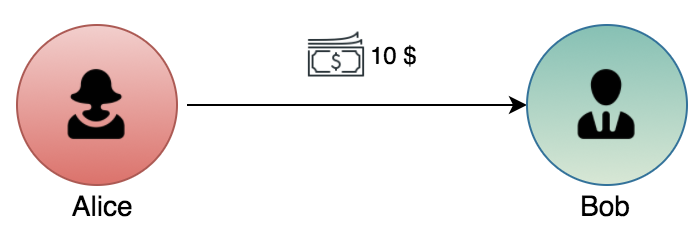
\includegraphics[width=8cm, keepaspectratio]{../images/cash.png}
    \caption{现金交割}
    \label{fig:cash}
\end{figure}

但是对于数字货币来讲,因为数字具有可复制性,而且成本几乎为零,所以双花问题就比较麻烦。
虽然数字签名技术可以确定所有者的身份,但是无法确定数字资产是否已经被花费。
回到上面的场景,Bob 可以通过数字签名可以验证 10 美元数字货币是 Alice 的,但是无法确认这 10 美元是否已经被 Alice 花费给了其他人。
这个问题的困难在于,Alice 可以把数字货币的所有权转给任何人,所以 Bob 需要访问所有可能的接受者,才能确认 Alice 之前没有花费这 10 美元。

\begin{figure}[h!]
    \centering
    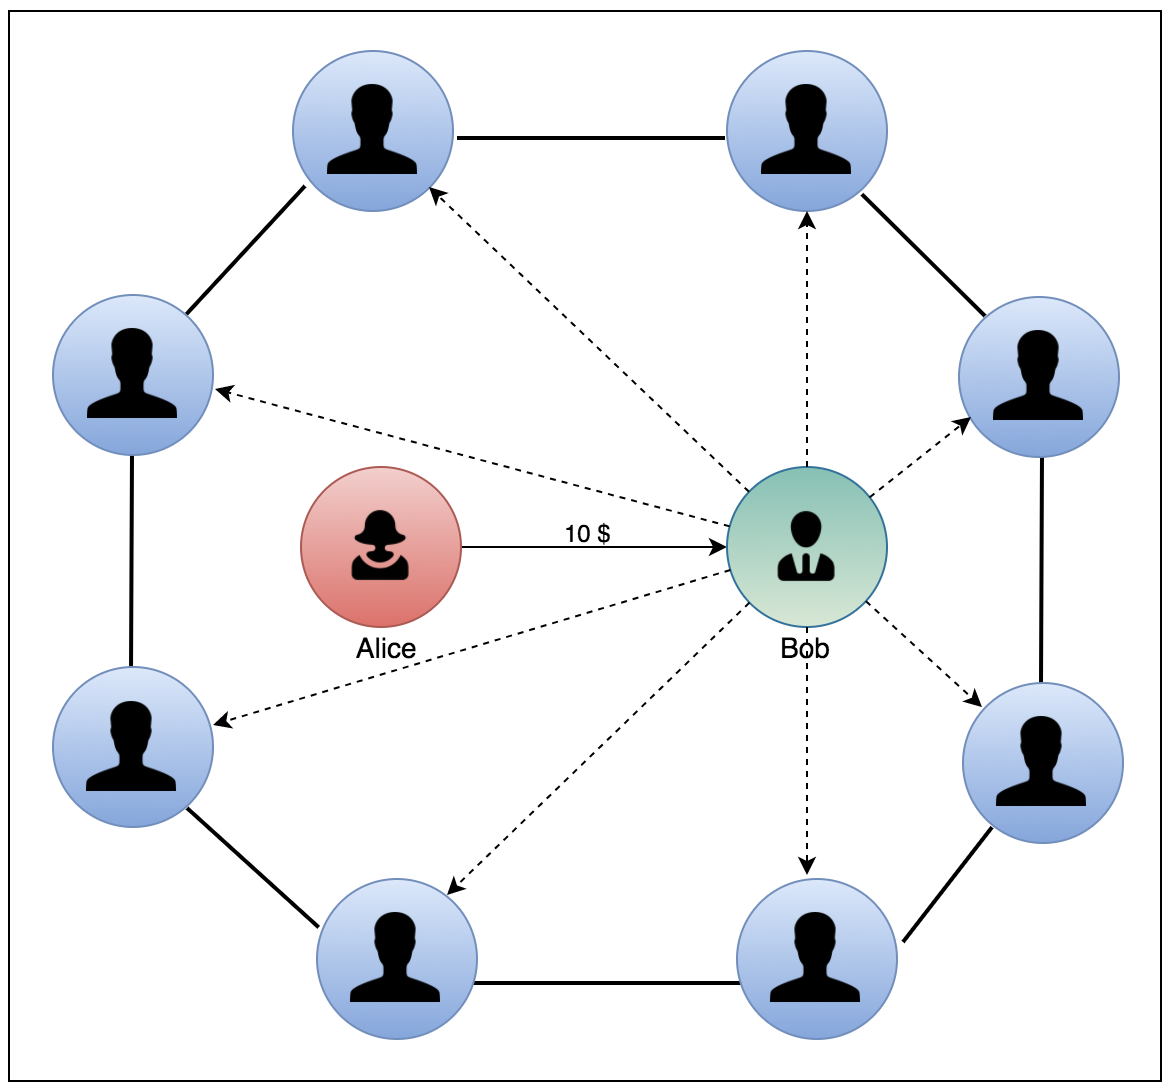
\includegraphics[width=8cm, keepaspectratio]{../images/Gossip_1.png}
    \caption{向所有人验证是否双花}
    \label{fig:gossip}
\end{figure}

显然穷举并且访问所有人是不可行的。对于这个问题,中本聪在比特币的创世论文中提到:

\begin{quote}
    \textbf{\textit{We need a way for the payee to know that the previous owners did not sign any earlier transactions. 
            For our purposes, the earliest transaction is the one that counts, so we don't care about later attempts to double-spend. 
            The only way to confirm the absence of a transaction is to be aware of all transactions.}}
\end{quote}

中本聪的解决办法是构建一个分布式共识账本,每一位独立的参与者都可以拥有一份副本。
副本中包含所有历史交易记录,这样 Bob 根据账本副本直接验证 Alice 是否已经花费了这 10 美元,免去了遍历所有的参与者的麻烦。

为了保证副本之间的一致性,每一笔交易都要交给矿工见证、附加上时间戳、按照先后顺序组成链式结构。
在见证的过程中附加上工作量证明,令攻击者必须要付出更多工作量才能篡改交易的历史记录。


比特币创造性的解决了数字货币的双花问题,经过10年的稳定运行,已经证明了其安全性。
但是这个解决方案存在天生的运行效率的瓶颈。比特币的平均吞吐量大约是 3~4 TPS,远远无法满足现代支付系统的需求。
回顾上面的分析,我们可以发现,问题的根源在于所有权的交割没有明确的范围限制,任何人可以把资产转移给任何人,所以每个人必须要保存所有的交易记录。
这其中包含的存储复杂度、通信复杂度、计算复杂度至少都是O(N)的,随着参与者数量 N 的增加,每笔交易的成本也增加。
无论系统怎么设计,都无法降低这些复杂度。

\subsection{债权的清算}

近代出现了银行、钱庄这样的组织,他们作为金融中介,可以通过债务清算的方式为用户提供支付服务。其工作原理如下图:

\begin{figure}[h!]
    \centering
    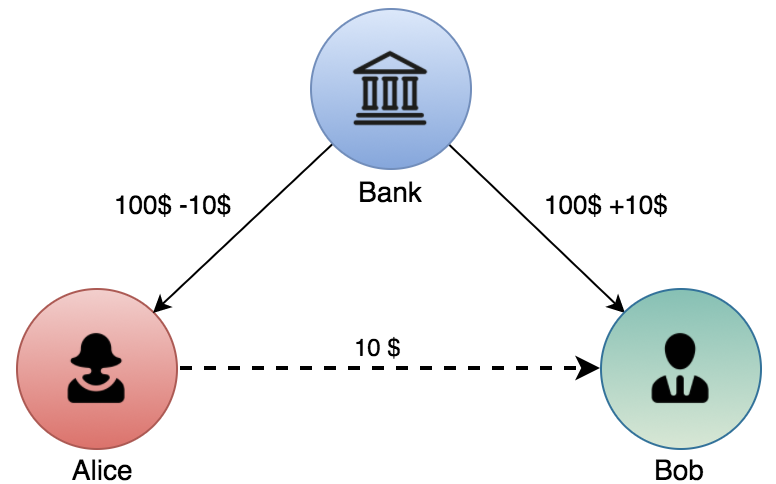
\includegraphics[width=8cm, keepaspectratio]{../images/clearing.png}
    \caption{通过债务清算完成支付}
    \label{fig:clearing}
\end{figure}

还是假设 Alice 要向 Bob 支付 10 美元,Alice 和 Bob 分别在银行里存入 100 美元。
或者说银行分别欠 Alice 和 Bob 100 美元。
当 Alice 需要向 Bob 支付 10 美元的时候,银行对 Alice 的债务余额减10美元,对 Bob 的债务余额加10美元。
支付过程中 不需要 Alice 和 Bob 之间交割任何实物货币,只需要银行居间调整债务余额就可以了。
在金融领域里,债务余额的调整的过程属于清算,债务终结的过程属于结算。
这种价值转移方式称之为:银行通过清算间接帮助 Alice 和 Bob 完成了结算。

因为相对于所有权交割的支付方式,债务清算的优势非常明显:

\begin{enumerate}
    \item 促进货币去实物化。
    
    虽然去实物化的过程从2千年前就开始了。
    货币从粮食、牲畜,发展到贵金属,再到纸钞,货币越来越轻便,内在价值越来越小。
    但是依然无法彻底脱离实物载体。
    到了债务货币阶段才彻底的变成数字。节省了保存、转移等成本。
    
    \item 自动化处理。
    
    数字化的债务货币非常适合计算机处理和网络传输。
    随着IT技术的发展,债务清算可以全自动化处理,并且可以支持随时随地的远程支付。
    
    \item 高效的规避双花问题。
    
    如果 Bob 要确认 Alice 没有双花,只需要让银行确认当前 Alice 的余额是否是最新的就可以了。
    不需要访问其它任何人就可以解决双花问题。相对于比特币协议,不需要 Gossip 通信让众多与交易无关的见证者参与共识。
    把通信、存储、计算复杂度从O(N)降到了 O(1)。
    大大提升了系统的效率,打破了比特币吞吐量的限制。
    
\end{enumerate}

通过可信的金融中介大大提高支付的效率、降低支付的摩擦,这种支付方式的创新几十年前就已经开始应用。
随着 Visa、支付宝、微信等支付系统的普及,获得了很大的成功。
但是这种方式也要付出代价。银行和客户之间的债务关系必须长期续存,这意味着客户的资产长期由银行托管。
银行必须有强大的信用背书和风控制度,防范道德风险、管理风险、信用风险,保证银行有充足的偿付能力,以免银行被挤兑。
为此现代金融系统建立了一整套法律和监管体系,防范这些风险的累积和爆发。
然而随着金融体系越来越庞大、越来越复杂,金融监管的成本也越来越高,这些成本最终转化交易的摩擦有消费者买单。

\subsection{总结}
我们从双花的视角总结一下所有权交割与债权清算。

\begin{itemize}
    \item 所有权交割是一对多的关系,支付的接收方必须检查所有人的交易记录才能解决双花问题,解决问题的复杂度是O(N)。
    \item 债权清算是一对一的关系,支付的接收方只需要银行确认对应的债务余额是最新的版本即可,解决问题的复杂度是O(1)。
\end{itemize}

所以可以得出结论,债权清算在双花问题上具有天然的优势。
如果要扩容比特币,与其在比特币协议上修修补补,不如切换价值转移的范式,改成债务清算的模式。
